% ##################################################################################################################
\section{Seoul}
\label{sec:seoul}
\hfill \textbf{Author:} Seungjae Lee, Atizaz Ali

% ##################################################################################################################
The \gls{matsim} model of \gls{sma} was developed in 2012 as a result of long-term research collaboration between the University of Seoul (Prof.\ Seungjae Lee) \& \gls{eth} Zürich (Prof.\ Kay W.\ Axhausen). The model was updated on a yearly basis and the demand is generated based on 2012 \gls{hhtsd}. The brief statistics related to the demand (input) are summarized as follows. 

The study area covers the \gls{sma} (Gyeonggi-do province with emphasis on Seoul Metro which comprises of 25\,main administrative districts). A population synthesizer was developed to generate the \gls{matsim} input demand based on \gls{hhtsd} 2012. Total population of \gls{sma} is 21.5\,million; therefore, a 10\,\% sample was generated and simulated (2.15\,million agents). A detailed network of nodes and links was generated capturing all the details (16\,384 nodes and 32\,768 links) for railways, highways, arterials, pedestrians, expressways and bus only lanes. \gls{emme2} network was converted to \gls{matsim} format. The 2012 Korean Transport Database was utilized to generate the transit schedules and vehicle definitions according to the bus types, railway and metro lines. Total number of routes is 1\,317 (contains regional buses, inter-city buses, feeder line buses and metro lines etc.). In collaboration with \gls{senozon}, a more realistic door-door demand was generated in Seoul City in July 2014. Data source is the Korean \gls{gis} department.

In Seoul context, \gls{matsim} has been widely used for various research purposes for policy evaluation, \citet[e.g.,][]{KimEtAl_IJHE_2012, LeeAli_unpub_IWUTSCD_2014}.

A master's thesis is currently underway by this section's second author looking at transit demand generation and calibration using smart card data in \gls{sma}. The work is sequenced as follows. A video is available form the authors on request.
%
\begin{compactitem}
\item Data mining (trimming off non-useful data)
\item	Converting disaggregate transactions (\gls{od}) to individual trips and trip segments based on user \lstinline|ID|
\item	Activities inference and assignment in \gls{spss} database
\item	Generating transit demand (\gls{matsim} input format)
\item	Updated transit network \& schedule for running the simulation
\item	Model calibration (in process)
\end{compactitem}
%
Moreover, \gls{matsim} tutorials are prepared for fall semester (2014) to help both undergrad and grad students at the Department of Transportation Engineering in getting working command at \gls{matsim}.

\createfigure%
{Seoul scenario}%
{Seoul scenario}%
{\label{fig:seoul}}%
{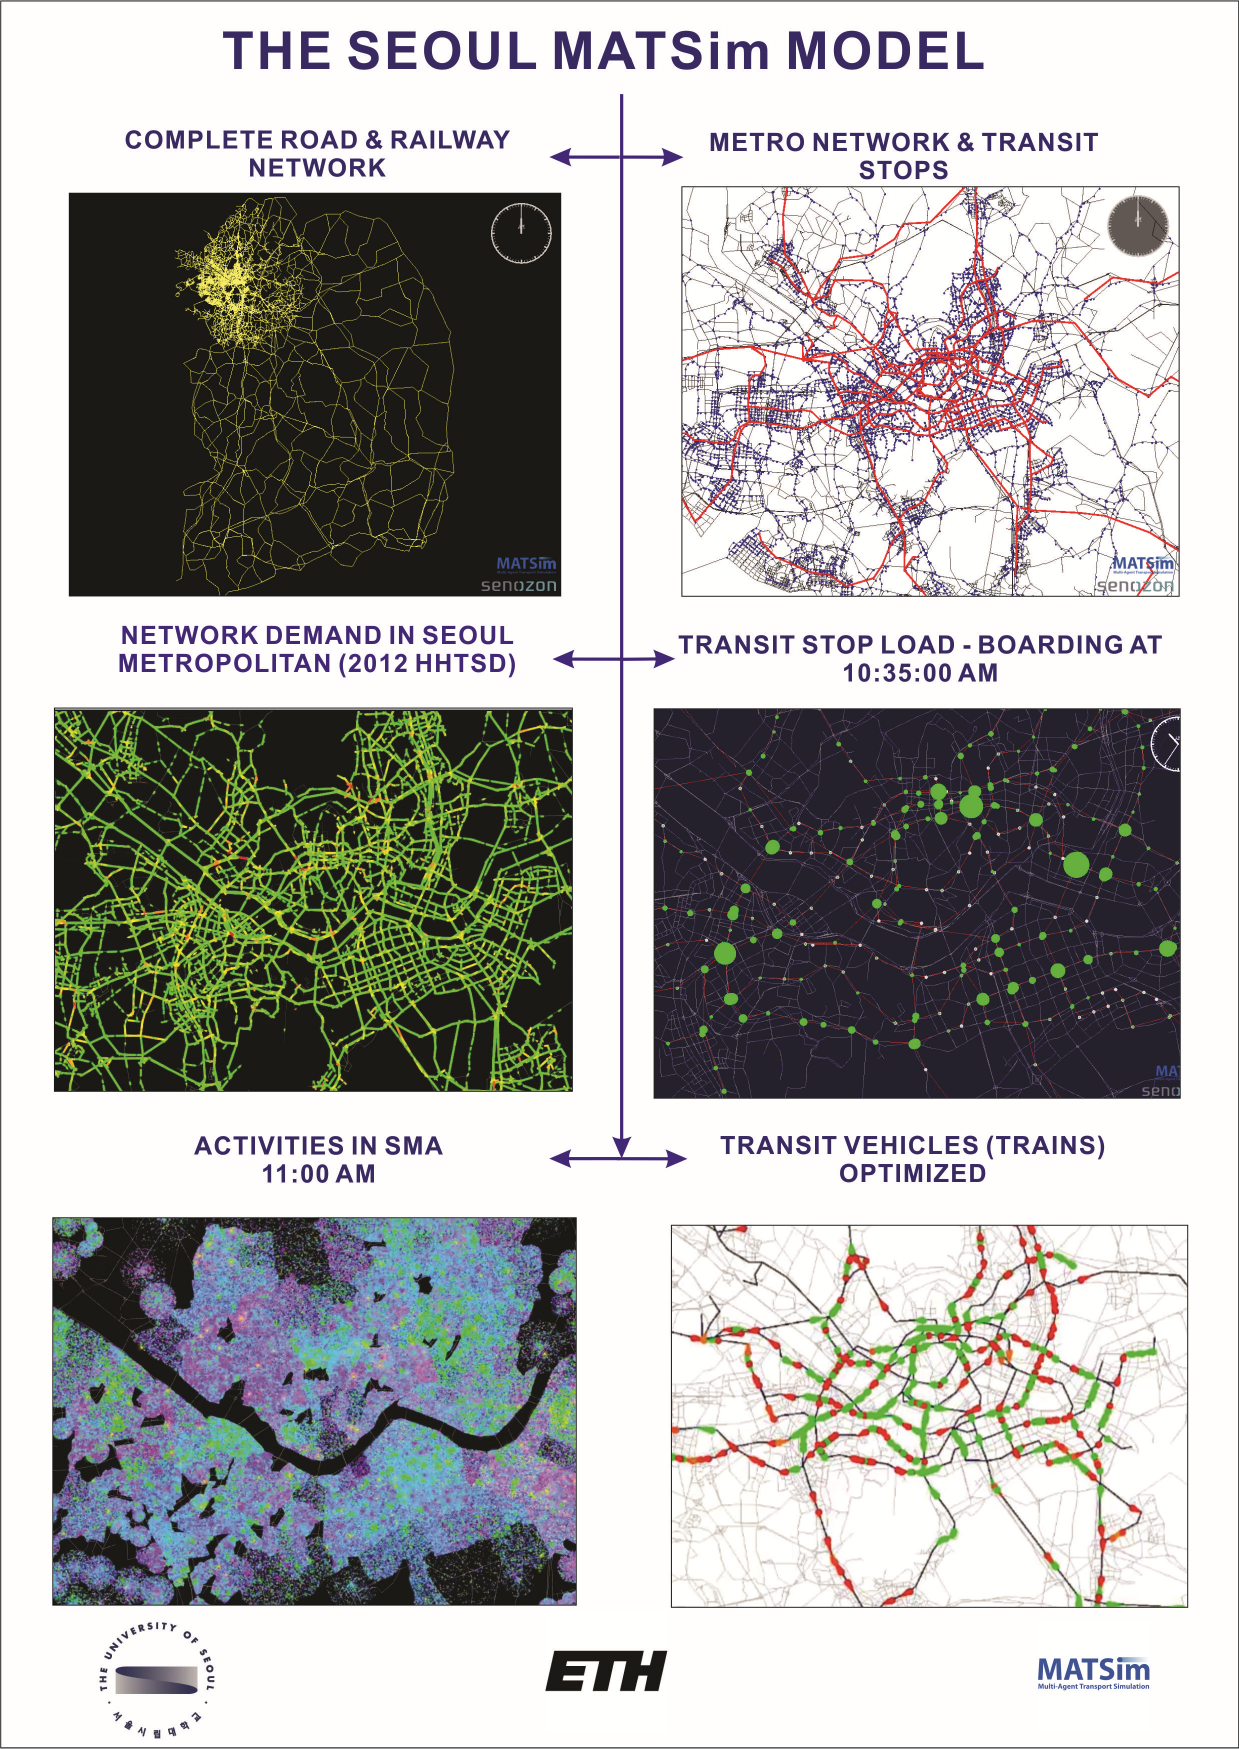
\includegraphics[width=0.99\textwidth, angle=0]{using/figures/seoul}}%
{}

% ##################################################################################################################
 
 
